%%
%% Qbe SAS SystemDocumentation
%% (C) Copyright 2001-2004 Christian Hofstaedtler
%%
%% $Id: part-last.tex 38 2004-05-12 13:59:31Z ch $
%%

\cChapter{Netzwerk�bersicht HTL}
�bersicht �ber die Server im HTL Netzwerk sowie der Anbindung an das Internet und die Clients.
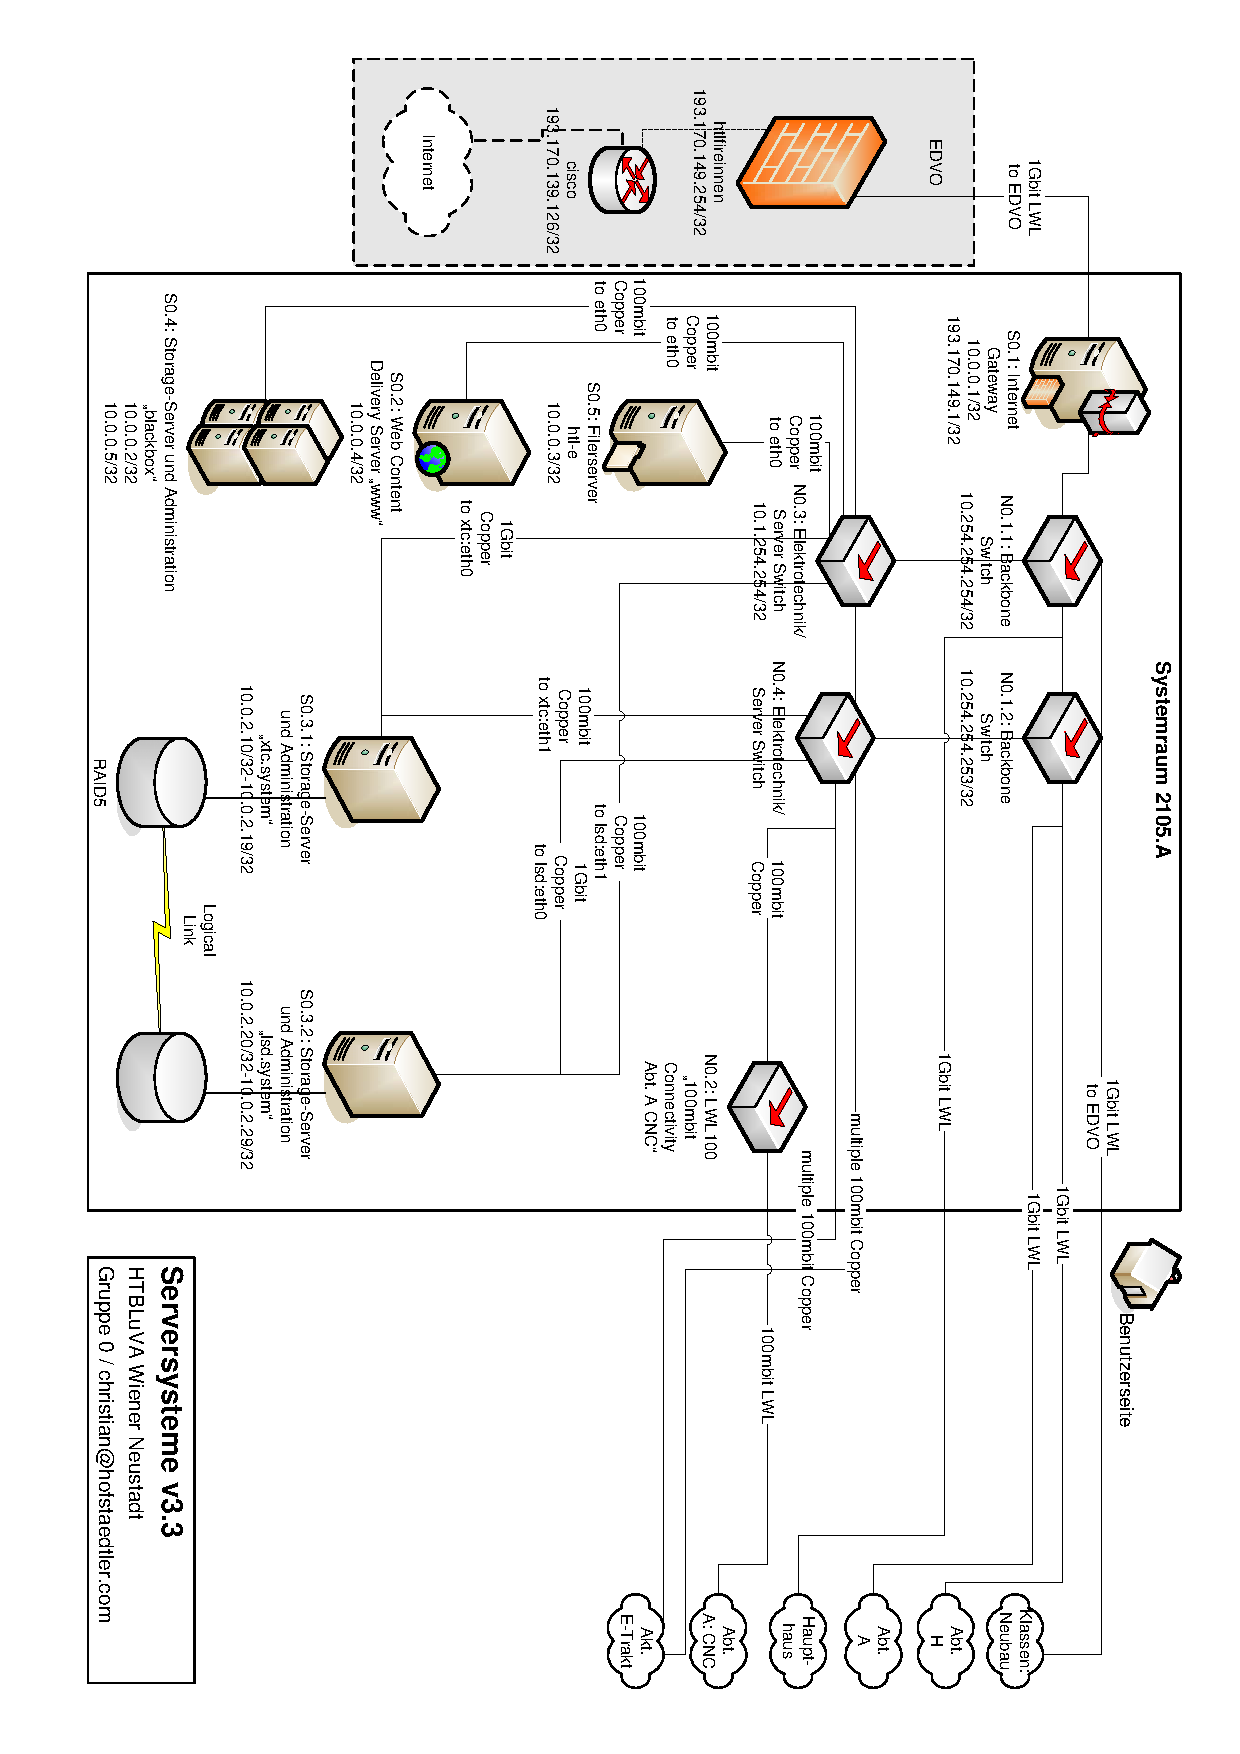
\includepdf[angle=90]{files/htl-net-struct.pdf}
%\{htl-net-struct.pdf}{HTL Netzwerkstruktur}

\cChapter{eDirectory Schema und Tree}
Die Qbe SAS Anwendung ben�tigt einige neue Attribute und Objekte. Diese Schemaerweiterungen wurden mit der OID Nummer der HTL angelegt.

\section{Neue eDirectory Attribute}

inetStatus, loggedonHost, loggedonMac, traffic und lastActivity werden in den Benutzer-, Gruppen-, Klassen-, und Computer-Objekten verwendet. Die qbePolicy*-Attribute werden nur f�r die Computer-Policy-Objekte (qbeHostPolicy) verwendet.

\begin{lstlisting}[
	classoffset=0,morekeywords={attributeTypes},keywordstyle=\color{QBlue},
	classoffset=1,morekeywords={NAME,SYNTAX,SINGLE-VALUE},keywordstyle=\color{QRed}
	]
attributeTypes: ( 1.2.826.0.1.16224.0.0.0.10 NAME 'inetStatus' SYNTAX 1.3.6.1.4.1.1466.115.121.1.27 SINGLE-VALUE )
attributeTypes: ( 1.2.826.0.1.16224.0.0.0.11 NAME 'loggedonHost' SYNTAX 1.3.6.1.4.1.1466.115.121.1.15{64512} SINGLE-VALUE )
attributeTypes: ( 1.2.826.0.1.16224.0.0.0.12 NAME 'loggedonMac' SYNTAX 1.3.6.1.4.1.1466.115.121.1.15{128} SINGLE-VALUE )
attributeTypes: ( 1.2.826.0.1.16224.0.0.0.13 NAME 'traffic' SYNTAX 1.3.6.1.4.1.1466.115.121.1.36{64512} SINGLE-VALUE )
attributeTypes: ( 1.2.826.0.1.16224.0.0.0.14 NAME 'lastActivity' SYNTAX 1.3.6.1.4.1.1466.115.121.1.27 SINGLE-VALUE )
attributeTypes: ( 1.2.826.0.1.16224.0.0.0.15 NAME 'qbePolicyDynamicUserGroup' SYNTAX 1.3.6.1.4.1.1466.115.121.1.15{64512} )
attributeTypes: ( 1.2.826.0.1.16224.0.0.0.16 NAME 'qbePolicyDynamicUserEnabled' SYNTAX 1.3.6.1.4.1.1466.115.121.1.27 SINGLE-VALUE )
attributeTypes: ( 1.2.826.0.1.16224.0.0.0.17 NAME 'qbePolicyName' SYNTAX 1.3.6.1.4.1.1466.115.121.1.12 )
attributeTypes: ( 1.2.826.0.1.16224.0.0.0.18 NAME 'qbePolicyLoginScript' SYNTAX 1.3.6.1.4.1.1466.115.121.1.15{64512} SINGLE-VALUE )
attributeTypes: ( 1.2.826.0.1.16224.0.0.0.19 NAME 'qbePolicyHomeDrive' SYNTAX1.3.6.1.4.1.1466.115.121.1.15{64512} SINGLE-VALUE )
attributeTypes: ( 1.2.826.0.1.16224.0.0.0.20 NAME 'qbePolicyHomeDriveDir' SYNTAX 1.3.6.1.4.1.1466.115.121.1.15{64512} SINGLE-VALUE )
\end{lstlisting}

Bei einer Neuinstallation sollten die Attribute inetStatus, loggedonHost, loggedonMac, traffic und lastActivity auf qbe* umbenannt werden. Dies w�rde die Schemaverwaltung vereinfachen, zieht jedoch auch �nderungen in den PHP Skripten nach sich.

\section{Neue eDirectory Objekte}

qbeOrganizationalUnit und qbeGroup werden f�r die Klassen-/Gruppen-Verwaltung verwendet. qbeIpDevice, qbeOwnedObject und qbeHostPolicy f�r die ComputerVerwaltung.

\begin{lstlisting}[%
	classoffset=0,morekeywords={objectClasses},keywordstyle=\color{QBlue},
	classoffset=1,morekeywords={NAME,SUP,MAY,MUST,AUXILIARY,X-NDS\_NOT\_CONTAINER},keywordstyle=\color{QRed},
	classoffset=2,morekeywords={\$},keywordstyle=\color{green}%
	]
objectClasses: ( 1.2.826.0.1.16224.0.0.0.1 NAME 'qbeOrganizationalUnit' SUP organizationalUnit AUXILIARY MAY ( cn $ inetStatus ) X-NDS_NOT_CONTAINER '1' )
objectClasses: ( 1.2.826.0.1.16224.0.0.0.2 NAME 'qbeGroup' SUP groupOfNames AUXILIARY MAY inetStatus X-NDS_NOT_CONTAINER '1' )

objectClasses: ( 1.2.826.0.1.16224.0.0.0.3 NAME 'qbeIpDevice' AUXILIARY MAY ( macAddress $ ipHostNumber $ qbePolicyName ) X-NDS_NOT_CONTAINER '1' )
objectClasses: ( 1.2.826.0.1.16224.0.0.0.4 NAME 'qbeOwnedObject' AUXILIARY MAY owner X-NDS_NOT_CONTAINER '1' )
objectClasses: ( 1.2.826.0.1.16224.0.0.0.5 NAME 'qbeHostPolicy' AUXILIARY MUST qbePolicyDynamicUserEnabled MAY ( qbePolicyDynamicUserGroup $ qbePolicyHomeDrive $ qbePolicyHomeDriveDir $ qbePolicyLoginScript ) X-NDS_NOT_CONTAINER '1' )
\end{lstlisting}

\section{eDirectory Tree �bersicht}
Im folgenden findet sich eine �bersicht des eDirectory Verzeichnisses. Hier mit Treename "HTL" und Basiskontext "o=htlwrn,c=at".

Der Kontext "o=System" ist nicht via \index{LDAP}{LDAP} sichtbar, kann daher auch nicht einfach von Applikationen ver�ndert/besch�digt werden.

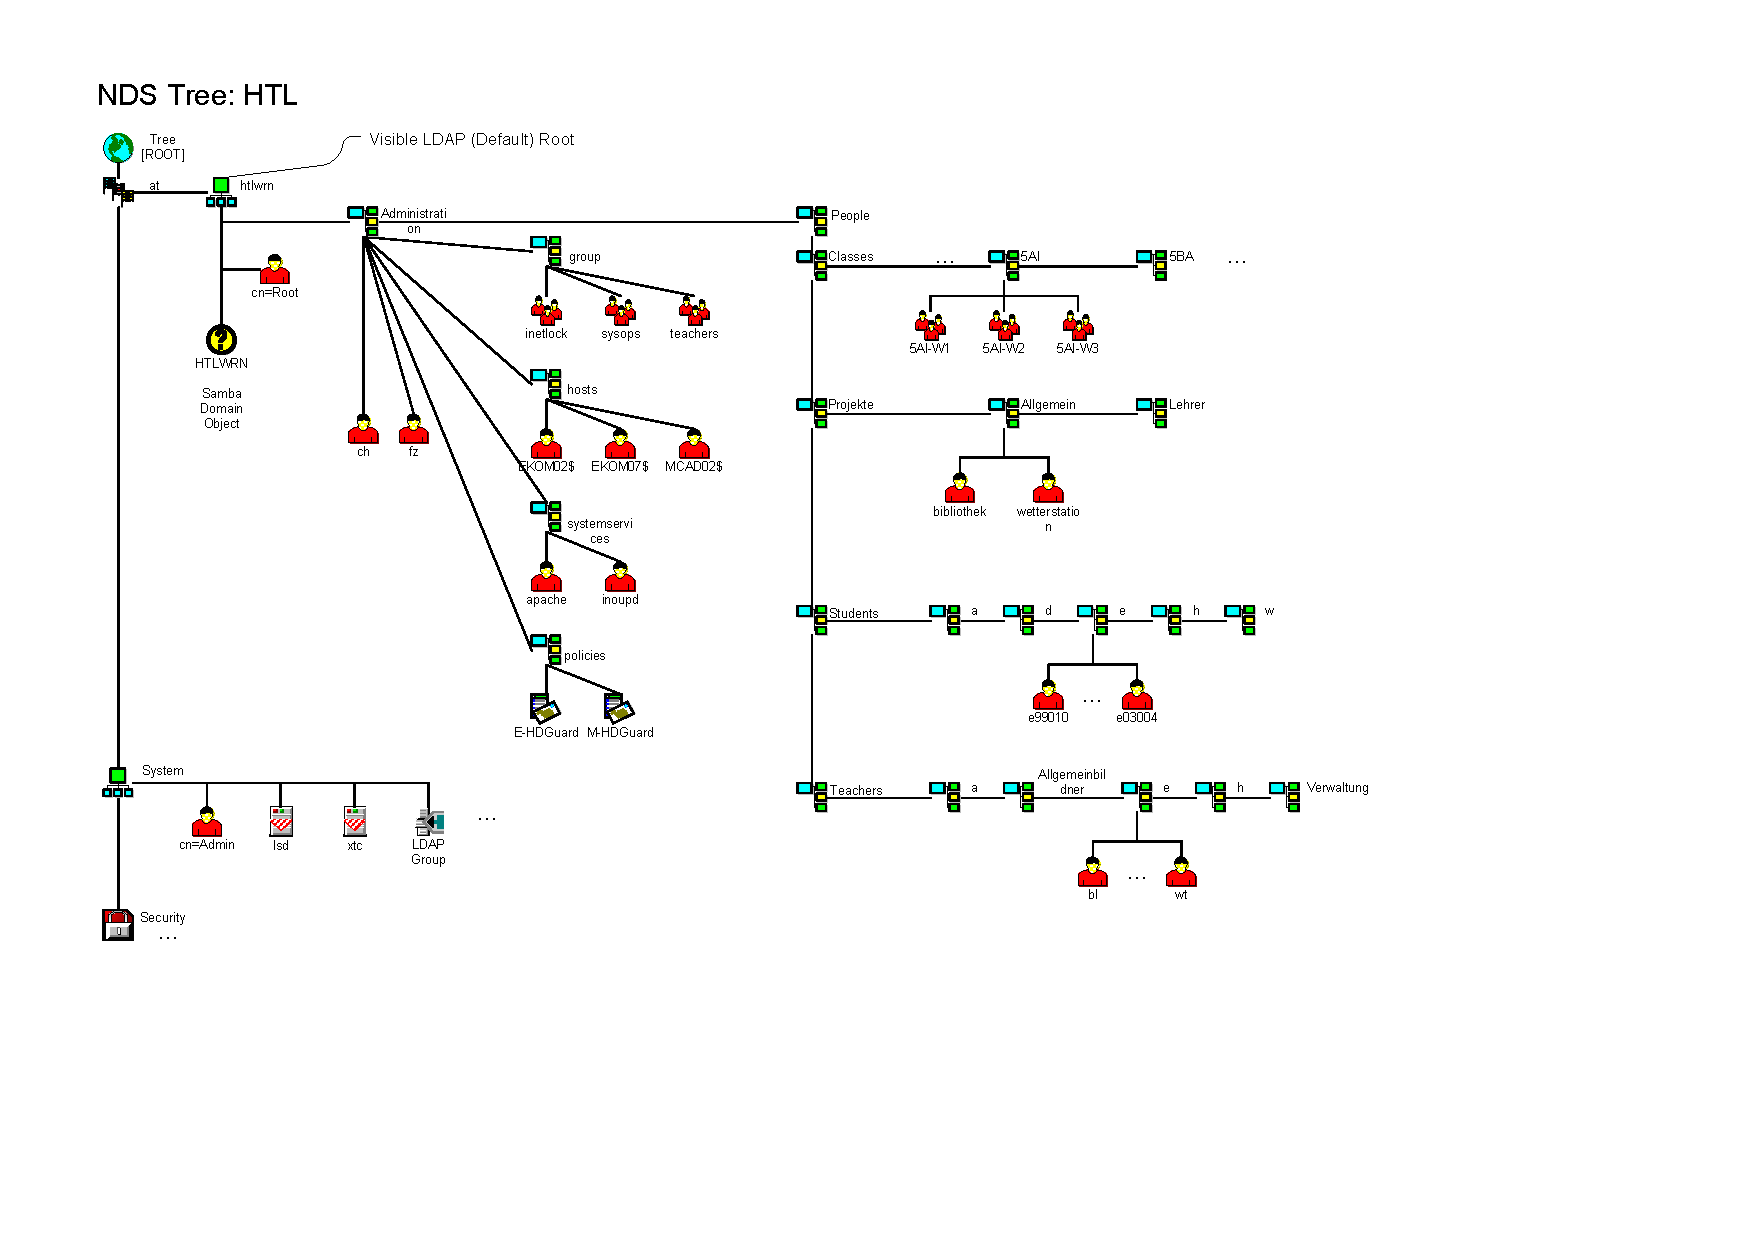
\includepdf[angle=90]{files/htl-nds-struct}
%{HTL eDirectory Struktur}
%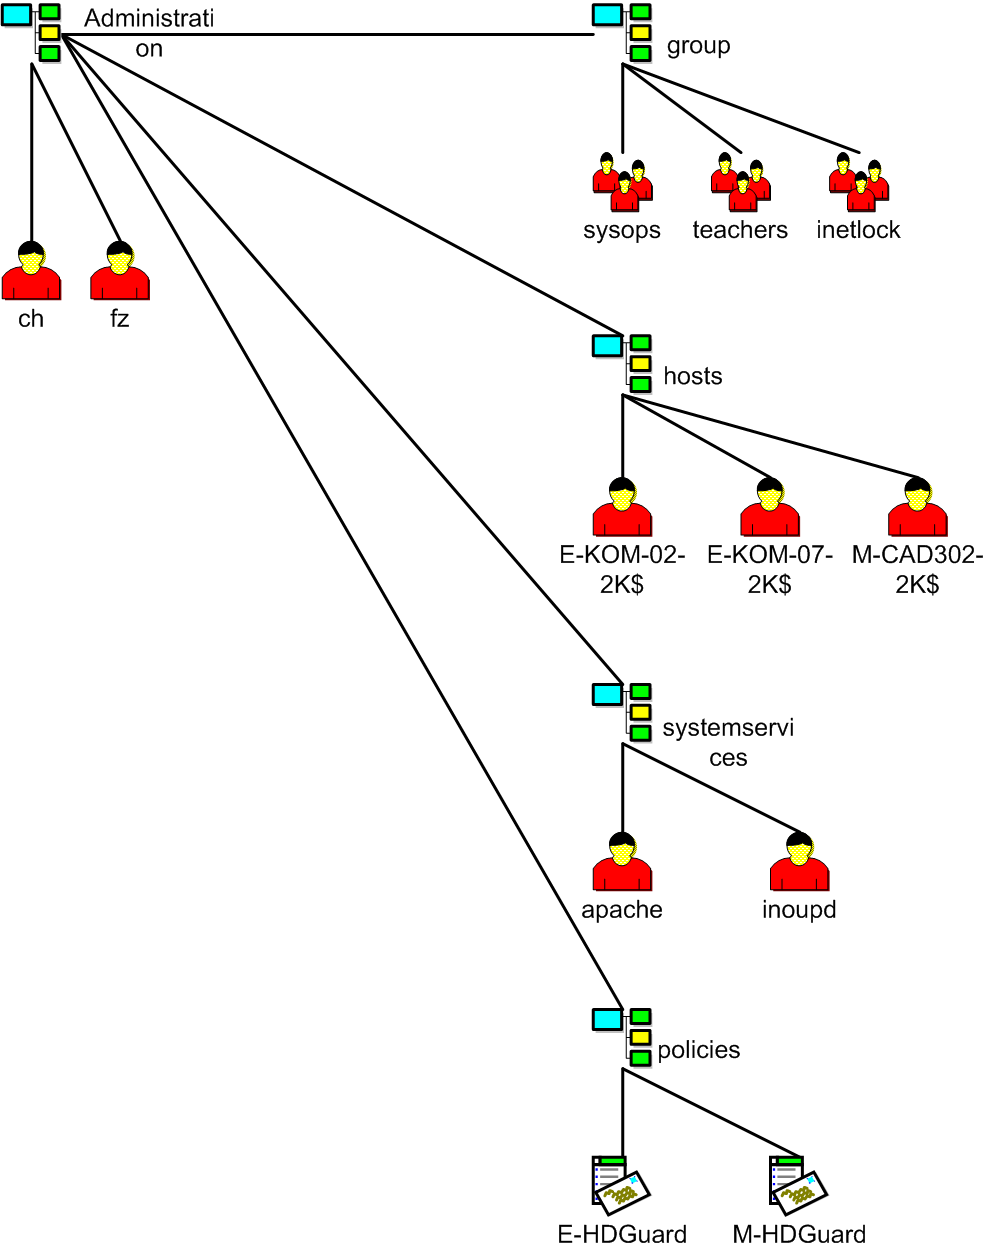
\includepdf[landscape]{files/htl-nds-struct-admin}

\par
\clearpage

\cChapter{Cluster-Installation HTL}

Der HTL-Cluster f�r den Authentication Server besteht aus zwei identischen Intel-Servern. Der Cluster-Name lautet auf qbe-auth.htlwrn.ac.at. Die Intel-Server wurden xtc.system.htlwrn.ac.at (Prim�rer Server) und lsd.system.htlwrn.ac.at (Sekund�rer Server) getauft.

Als Cluster Monitor-Software wird heartbeat eingesetzt. Die Intel-Server sind vom Modell SR2300 und mit dem Intel SE7501WV2 sowie dem Intel Raid-Controller SRCZCR ausgestattet. Je Server sind 5 Seagate 73GB SCSI Hotswap Disks eingebaut und werden als RAID 5 mit Hotspare verwendet.

Novell eDirectory wird nicht vom heartbeat verwaltet, es l�uft immer auf beiden Cluster Nodes. Alle anderen Dienste werden vom heartbeat gestartet/gestoppt.

Um das Daten-Volume \verb|/raid| auf beiden Cluster-Nodes konsistent zu halten, wird ein Netzwerk-RAID1 mit drbd aufgebaut. Damit wird nicht direkt die Partition \verb|/dev/sda7| sondern das drbd Device \verb|/dev/nb0| gemountet. Als Filesystem wird journaling ext3 eingesetzt.

Partitionen:
\begin{lstlisting}[language=]
Device    Boot  Id  Type
/dev/sda1       12  System Diagnostics
/dev/sda2  *    83  Linux          /boot (ext2)
/dev/sda3        5  Extended
/dev/sda5       83  Linux          / (ext3)
/dev/sda6       82  Linux swap
/dev/sda7       83  Linux          /raid via drbd (ext3)
\end{lstlisting}


Konfiguration Netzwerk-RAID1 /etc/drbd.conf:
\begin{lstlisting}
resource drbd0 {
  protocol=A			# Protokolltyp A
  fsckcmd=fsck.ext3 -p -y	# ext3 fsck verwenden
  disk {
        disk-size=132255081	# Partition Objektgroesse in Byte
  }
  net {
    sync-rate=100000		# Maximale Synchronisationsgeschwindigkeit
  }
  on xtc {
    device=/dev/nb0
    disk=/dev/sda7		# Partitiondevice
    address=192.168.177.1	# IP Adresse des ersten Clusternode
    port=7788
  }
  on lsd {
    device=/dev/nb0
    disk=/dev/sda7		# Partitiondevice
    address=192.168.177.2	# IP Adresse der zweiten Clusternode
    port=7788
  }
}
\end{lstlisting}

Die Cluster-Applikationen und IP-Adressen:
\begin{description}
\item[Filesystem::/dev/nb0::/raid::ext3::noatime,usrquota,grpquota]{Das /raid Datendateisystem}
\item[qbe-sas-daemon]{Hintergrunddienste vom Application Server}
\item[10.0.2.100]{Application Server IP-Adresse}
\item[172.16.0.1/16]{Application Server IP f�r unbekannte Clients}
\item[apache::/etc/apache/httpd.conf]{Application Server Webserver}
\item[samba]{CIFS Server}
\item[mysql]{SQL Server}
\item[vsftpd]{FTP Server}
\item[nfs-kernel-server]{Network File System (NFS) Server f�r die www}
\item[dhcp3-server]{DHCP Server}
\item[10.0.2.104]{SubVersion IP-Adresse}
\item[apache2]{SubVersion Server}
\end{description}


%% *eof*

